%#################################################################
\chapter{Mapeamento Multivocal de Literatura}\label{mapeamentoLiteratura}
%#################################################################

Esse capítulo descreve os procedimentos adotados para a investigação da literatura realizada para este estudo. 
Para este propósito ser alcançado foi realizado o planejamento e a execução de um Mapeamento Multivocal da Literatura, do inglês \ac{MLM}. 
Para isto foram aplicadas diretrizes bem estabelecidas conceitualmente por diversos trabalhos \cite{Kitchenham:2007, Petersen:2008, Nakagawa:2017}.  

O protocolo seguido é descrito de forma detalhada na Seção \ref{sec:Protocolo}. 
%Na Subseção \ref{ssec:QPs} são elencadas as nossas \ac{QP}, as fontes de busca na Subseção \ref{ssec:FontesBuscas}. 
%Na Subseção \ref{ssec:StringBusca} apresenta-se os termos e a \textit{string} gerada a partir deles. 
%Os critérios de seleção são categorizados em \acp{CI} e \acp{CE} na Subseção \ref{ssec:CritSelecao}. 
%A avaliação de qualidade feita nos estudos primários é explicada na Subseção \ref{tab:AvalQualidade}. 
%Na Subseção \ref{ssec:EstratExtDados} são especificados os dados que deveriam ser observados nos estudos, caracterizando nossa estratégia de extração de dados. 
Na Seção \ref{sec:ExecMapeamento} é relatado todo o processo de execução do mapeamento multivocal. 
Os resultados provenientes da execução são analisados e discutidos na Seção \ref{sec:ResultDis}. 
As ameaças ao \ac{MLM} são debatidas na Seção \ref{sec:AmeacaVal} e, por fim, são pontuadas algumas lições do capítulo na Seção \ref{sec:LicoesMapeamento}.


%#################################################################
\section{Protocolo} \label{sec:Protocolo}
%#################################################################

Um \ac{MLM} é uma forma de Mapeamento Sistemático de Literatura, do inglês \ac{SLM}, que inclui a literatura cinza. 
Os \acp{MLM} são úteis para pesquisadores e para profissionais pois fornecem visões abrangentes sobre o estado da arte e da prática em uma determinada área. 
Neste estudo conduziu-se um \ac{MLM} utilizando o processo de \ac{SLM} definido por Petersen~\cite{Petersen:2008} e as diretrizes propostas por \citeonline{Garousi:2019} para pesquisa na literatura cinza.

Um \ac{SLM} envolve uma busca para determinar que tipos de estudos abordam as questões de pesquisa que se objetiva investigar, além de possibilitar a classificação e extração de dados que possam gerar informações relevantes~\cite{Bailey:2007}. 
Com o propósito de ter a obtenção de resultados confiáveis e reproduzíveis em um \ac{SLM}, é vital que uma série de atividades bem definidas e estruturadas sejam seguidas \cite{Nakagawa:2017}. 
Na \autoref{fig:SystematicMappingProcess} é apresentado o processo de \ac{SLM} realizado neste estudo, com base na proposição realizada por \citeonline{Petersen:2008}. %Em linhas gerais este processo define todas as etapas necessárias para conduzir o \ac{SLM}. 
%Isso compreende a delimitação das \acp{QP}, a escolha das bases a serem utilizadas, a aplicação dos critérios de seleção, a estratégia de leitura e extração de dados dos estudos, a avaliação de qualidade e a síntese dos resultados obtidos.

\begin{figure}[htb]
	\centering
	\caption{Processo de mapeamento sistemático.}
		%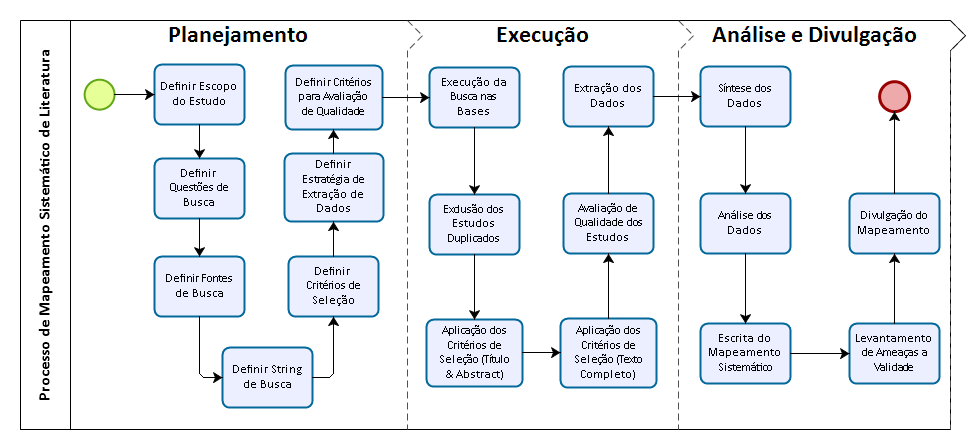
\includegraphics[width=\textwidth]{img/ProcessoMSL.png}
		\tikzset{every picture/.style={line width=0.75pt}} %set default line width to 0.75pt        

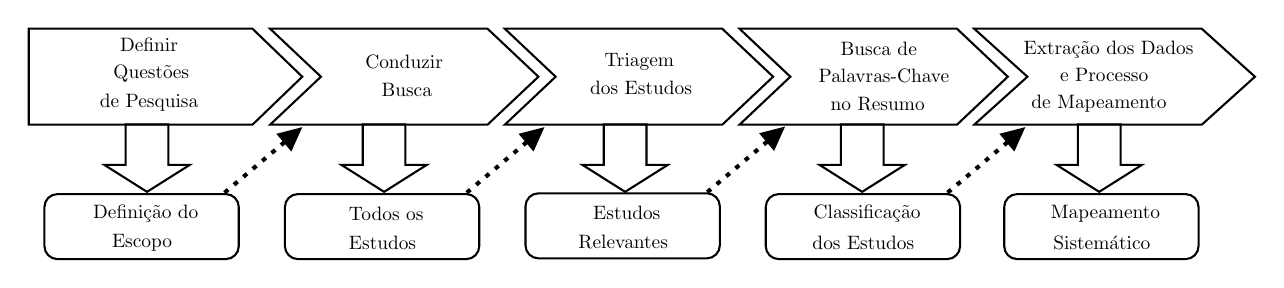
\begin{tikzpicture}[x=0.75pt,y=0.75pt,yscale=-1,xscale=1]
%uncomment if require: \path (0,295); %set diagram left start at 0, and has height of 295

%Pentagon Arrow [id:dp6278377926239387] 
\draw   (53.7,53) -- (161.5,53) -- (185.5,76.13) -- (161.5,99.25) -- (53.7,99.25) -- cycle ;
%Chevron Arrow [id:dp8061814950023936] 
\draw   (169.99,53) -- (274.76,53) -- (299.27,76.13) -- (274.76,99.25) -- (169.99,99.25) -- (194.5,76.13) -- cycle ;
%Chevron Arrow [id:dp5292331748785577] 
\draw   (283.07,53) -- (387.84,53) -- (412.35,76.13) -- (387.84,99.25) -- (283.07,99.25) -- (307.58,76.13) -- cycle ;
%Chevron Arrow [id:dp23027191263172608] 
\draw   (509.23,53) -- (618.86,53) -- (644.5,76.13) -- (618.86,99.25) -- (509.23,99.25) -- (534.87,76.13) -- cycle ;
%Chevron Arrow [id:dp12330558695774196] 
\draw   (396.15,53) -- (500.92,53) -- (525.42,76.13) -- (500.92,99.25) -- (396.15,99.25) -- (420.65,76.13) -- cycle ;
%Rounded Rect [id:dp4602302829049887] 
\draw   (61.27,138.93) .. controls (61.27,135.47) and (64.08,132.67) .. (67.54,132.67) -- (148.65,132.67) .. controls (152.11,132.67) and (154.91,135.47) .. (154.91,138.93) -- (154.91,157.73) .. controls (154.91,161.19) and (152.11,164) .. (148.65,164) -- (67.54,164) .. controls (64.08,164) and (61.27,161.19) .. (61.27,157.73) -- cycle ;
%Rounded Rect [id:dp8032081633216976] 
\draw   (523.69,138.93) .. controls (523.69,135.47) and (526.5,132.67) .. (529.96,132.67) -- (611.07,132.67) .. controls (614.53,132.67) and (617.33,135.47) .. (617.33,138.93) -- (617.33,157.73) .. controls (617.33,161.19) and (614.53,164) .. (611.07,164) -- (529.96,164) .. controls (526.5,164) and (523.69,161.19) .. (523.69,157.73) -- cycle ;
%Rounded Rect [id:dp3313220993143424] 
\draw   (408.8,138.93) .. controls (408.8,135.47) and (411.6,132.67) .. (415.06,132.67) -- (496.17,132.67) .. controls (499.63,132.67) and (502.44,135.47) .. (502.44,138.93) -- (502.44,157.73) .. controls (502.44,161.19) and (499.63,164) .. (496.17,164) -- (415.06,164) .. controls (411.6,164) and (408.8,161.19) .. (408.8,157.73) -- cycle ;
%Rounded Rect [id:dp4120899111688079] 
\draw   (293.04,138.57) .. controls (293.04,135.11) and (295.84,132.3) .. (299.3,132.3) -- (380.41,132.3) .. controls (383.87,132.3) and (386.68,135.11) .. (386.68,138.57) -- (386.68,157.37) .. controls (386.68,160.83) and (383.87,163.64) .. (380.41,163.64) -- (299.3,163.64) .. controls (295.84,163.64) and (293.04,160.83) .. (293.04,157.37) -- cycle ;
%Rounded Rect [id:dp45930303754942536] 
\draw   (177.13,138.93) .. controls (177.13,135.47) and (179.94,132.67) .. (183.4,132.67) -- (264.5,132.67) .. controls (267.97,132.67) and (270.77,135.47) .. (270.77,138.93) -- (270.77,157.73) .. controls (270.77,161.19) and (267.97,164) .. (264.5,164) -- (183.4,164) .. controls (179.94,164) and (177.13,161.19) .. (177.13,157.73) -- cycle ;
%Down Arrow [id:dp3807248413929003] 
\draw  [line width=0.75]  (90.13,118.6) -- (100.42,118.6) -- (100.42,99.1) -- (121,99.1) -- (121,118.6) -- (131.3,118.6) -- (110.71,131.6) -- cycle ;
%Down Arrow [id:dp47792969981808375] 
\draw  [line width=0.75]  (204.34,118.6) -- (214.63,118.6) -- (214.63,99.1) -- (235.21,99.1) -- (235.21,118.6) -- (245.5,118.6) -- (224.92,131.6) -- cycle ;
%Down Arrow [id:dp6527476506757643] 
\draw  [line width=0.75]  (320.47,118.6) -- (330.76,118.6) -- (330.76,99.1) -- (351.34,99.1) -- (351.34,118.6) -- (361.63,118.6) -- (341.05,131.6) -- cycle ;
%Down Arrow [id:dp6109879640313591] 
\draw  [line width=0.75]  (434.68,118.6) -- (444.97,118.6) -- (444.97,99.1) -- (465.55,99.1) -- (465.55,118.6) -- (475.84,118.6) -- (455.26,131.6) -- cycle ;
%Down Arrow [id:dp08052269206416462] 
\draw  [line width=0.75]  (548.88,118.6) -- (559.17,118.6) -- (559.17,99.1) -- (579.75,99.1) -- (579.75,118.6) -- (590.04,118.6) -- (569.46,131.6) -- cycle ;
%Straight Lines [id:da6425776226592788] 
\draw [line width=1.5]  [dash pattern={on 1.69pt off 2.76pt}]  (148.07,132) -- (183.21,102.37) ;
\draw [shift={(185.5,100.43)}, rotate = 499.86] [fill={rgb, 255:red, 0; green, 0; blue, 0 }  ][line width=1.5]  [draw opacity=0] (11.61,-5.58) -- (0,0) -- (11.61,5.58) -- cycle    ;

%Straight Lines [id:da624041708353656] 
\draw [line width=1.5]  [dash pattern={on 1.69pt off 2.76pt}]  (264.75,132) -- (299.89,102.37) ;
\draw [shift={(302.18,100.43)}, rotate = 499.86] [fill={rgb, 255:red, 0; green, 0; blue, 0 }  ][line width=1.5]  [draw opacity=0] (11.61,-5.58) -- (0,0) -- (11.61,5.58) -- cycle    ;

%Straight Lines [id:da30892482975542945] 
\draw [line width=1.5]  [dash pattern={on 1.69pt off 2.76pt}]  (380.65,131.73) -- (415.79,102.1) ;
\draw [shift={(418.09,100.16)}, rotate = 499.86] [fill={rgb, 255:red, 0; green, 0; blue, 0 }  ][line width=1.5]  [draw opacity=0] (11.61,-5.58) -- (0,0) -- (11.61,5.58) -- cycle    ;

%Straight Lines [id:da19825567767990848] 
\draw [line width=1.5]  [dash pattern={on 1.69pt off 2.76pt}]  (496.41,132) -- (531.56,102.37) ;
\draw [shift={(533.85,100.43)}, rotate = 499.86] [fill={rgb, 255:red, 0; green, 0; blue, 0 }  ][line width=1.5]  [draw opacity=0] (11.61,-5.58) -- (0,0) -- (11.61,5.58) -- cycle    ;


% Text Node
\draw (111.66,60.53) node [scale=0.7] [align=left] {Definir};
% Text Node
\draw (112.75,74.83) node [scale=0.7] [align=left] {Questões};
% Text Node
\draw (111.66,88.6) node [scale=0.7] [align=left] {de Pesquisa};
% Text Node
\draw (234.55,68.76) node [scale=0.7] [align=left] {Conduzir};
% Text Node
\draw (235.84,82.37) node [scale=0.7] [align=left] {Busca};
% Text Node
\draw (347.88,68.76) node [scale=0.7] [align=left] {Triagem};
% Text Node
\draw (348.71,81.64) node [scale=0.7] [align=left] {dos Estudos};
% Text Node
\draw (463.25,62.65) node [scale=0.7] [align=left] {Busca de};
% Text Node
\draw (465.75,75.78) node [scale=0.7] [align=left] {Palavras-Chave};
% Text Node
\draw (462.75,89.1) node [scale=0.7] [align=left] {no Resumo};
% Text Node
\draw (573.99,63) node [scale=0.7] [align=left] {Extração dos Dados};
% Text Node
\draw (571.87,75.27) node [scale=0.7] [align=left] {e Processo};
% Text Node
\draw (569.37,89.19) node [scale=0.7] [align=left] {de Mapeamento};
% Text Node
\draw (110.09,142.14) node [scale=0.7] [align=left] {Definição do};
% Text Node
\draw (108.31,155.98) node [scale=0.7] [align=left] {Escopo};
% Text Node
\draw (572.51,142.14) node [scale=0.7] [align=left] {Mapeamento};
% Text Node
\draw (570.74,155.98) node [scale=0.7] [align=left] {Sistemático};
% Text Node
\draw (457.62,142.14) node [scale=0.7] [align=left] {Classificação};
% Text Node
\draw (455.84,155.98) node [scale=0.7] [align=left] {dos Estudos};
% Text Node
\draw (341.85,141.77) node [scale=0.7] [align=left] {Estudos};
% Text Node
\draw (340.08,155.62) node [scale=0.7] [align=left] {Relevantes};
% Text Node
\draw (225.95,142.14) node [scale=0.7] [align=left] {Todos os};
% Text Node
\draw (224.17,155.98) node [scale=0.7] [align=left] {Estudos};


\end{tikzpicture}
	\fonte{Adaptado de \citeonline{Petersen:2008}.}
	\label{fig:SystematicMappingProcess}
\end{figure}

%#################################################################
    \subsection{Questões de Pesquisa} \label{ssec:QPs}
%#################################################################

Levando-se em consideração o objetivo geral deste trabalho, o qual é desenvolver uma \ac{DSL} para a modelagem conceitual de \acp{BD}, foram formulados os seguintes questionamentos que serviram de guia para o restante do \ac{MLM}:

\begin{itemize}
    \small
    \item \textbf{QP1.}: Qual o estado da arte do desenvolvimento de DSLs para transformação de modelos em ER?
    \item \textbf{QP1.1.}: Quais são as metodologias, técnicas e propostas de refinamento (desenho automatizado) baseado em modelos de dados?
    \item \textbf{QP1.2.}: Qual é o ferramental utilizado como apoio ao desenvolvimento dessas DSL?
    \item \textbf{QP1.3.}: Quais são as representações de objetos de \ac{BD} adotadas ou sugeridas nas DSL propostas?
    \item \textbf{QP2} Quais os métodos de avaliação utilizados nos estudos?
    \item \textbf{QP2.1.}: Quais os pontos positivos e negativos observados na execução dos estudos?
    \item \textbf{QP2.2.}: Quais desafios são apontados após execução dos estudos empíricos?
    \item \textbf{QP3.}: Quais são as ferramentas para modelagem conceitual de \acp{BD}? 
    \item \textbf{QP3.1.}: Quais são as notações que estas ferramentas usam?
    \item \textbf{QP3.2.}: Quais são os níveis de modelagem de \ac{BD} (Conceitual, Lógico, Físico) que estas ferramentas suportam?
\end{itemize}

%#################################################################
    \subsection{Fontes de Busca} \label{ssec:FontesBuscas}
%#################################################################

As bibliotecas digitais são a principal fonte de busca em um \ac{SLM} \cite{Petersen:2008}. 
Para a escolha das fontes de busca desse \ac{SLM} são considerados três requisitos obrigatórios que as bases devem contemplar: 
\textbf{(I)} possuir mecanismo de pesquisa baseado na \textit{Web}; 
\textbf{(II)} ser capaz de usar palavras-chave durante a pesquisa, e;
\textbf{(III)} abranger estudos primários da grande área da Ciência da Computação. 
Na \autoref{tab:BasesDePesquisa} são listadas as bibliotecas digitais selecionadas para este \ac{SLM}.
        
\rowcolors{1}{gray!15}{white}
\begin{table}[!ht]
    \centering
    \footnotesize
    \caption{Bibliotecas digitais utilizadas.}
    \label{tab:BasesDePesquisa}
    \begin{tabular}{m{4cm}m{4cm}m{4cm}}
    \bottomrule
    \rowcolor[HTML]{C0C0C0}
    \textbf{Fonte} & \textbf{Endereço} & \textbf{Tipo} \\ 
    \hline
    ACM Digital library & \textit{dl.acm.org}           & Híbrida\\
    IEEE Xplore         & \textit{ieeexplore.ieee.org}  & Base Bibliográfica \\ 
    ScienceDirect       & \textit{sciencedirect.com}    & Base Bibliográfica \\
    Scopus       & \textit{scopus.com}   & Motor de Busca \\
    SpringerLink        & \textit{link.springer.com}    & Base Bibliográfica \\ 
    \bottomrule
    \end{tabular}
    \fonte{Adaptado de \citeonline{Nakagawa:2017}.}
\end{table}
            
%#################################################################
    \subsection{String de Busca} \label{ssec:StringBusca}
%#################################################################

A elaboração da \textit{string} de busca não é uma tarefa trivial. 
A identificação de uma combinação de termos que permitam encontrar o maior número de estudos primários relevantes de forma objetiva necessita, na maioria dos casos, de experiência e profundo conhecimento sobre a área de pesquisa abordada.  

\rowcolors{1}{gray!15}{white}
\begin{table}[!h]
    \centering
    \small
    \caption{Termos e sinônimos utilizados.}
    \label{tab:DefinicaoSearch}
    \begin{tabular}{m{4.5cm}m{10.5cm}}
        \bottomrule
        \rowcolor[HTML]{C0C0C0}
        \textbf{Termos} & \textbf{Sinônimos}\\
        \hline
        Domain Specific Language & DSL, Domain-Specific Language, Domain-Specific-Language, DSLM, Domain Specific Modeling Language, Domain-Specific Modeling Language, Domain-Specific-Modeling-Language, Query Language \\
        \hline
        Entity-Relationship & ER, Enhanced Entity-Relationship, EER, Database \\
        \toprule
    \end{tabular}
    \fonte{O autor.}
\end{table}
        
Para a formação da \textit{string} de busca é fundamental definir um conjunto de palavras referentes ao tema de pesquisa, bem como os sinônimos considerados expressivos. 
Estes termos devem representar de forma abrangente o tema central do estudo. 
Para este trabalho foram estabelecidos os termos e sinônimos da \autoref{tab:DefinicaoSearch}, sendo que sua combinação gerou a \textit{string} genérica da \autoref{fig:StringBusca}.
        
\begin{figure}[htb]
    \caption{String genérica de busca.}
    \centering
    \small
    \fbox{
    \parbox{14cm}{
    \centering
    \small\texttt{
    (DSL OR Domain Specific Language OR Domain-Specific Language OR Domain-Specific-Language OR DSLM OR Domain Specific Modeling Language OR Domain-Specific Modeling Language OR Domain-Specific-Modeling-Language OR Query Language)
    AND 
    (ER OR Entity-Relationship OR Enhanced Entity-Relationship OR Extended Entity-Relationship OR Database)
    }}}
    \fonte{O autor.}
    \label{fig:StringBusca}
\end{figure}
        
%#################################################################
    \subsection{Critérios de Seleção} \label{ssec:CritSelecao}
%#################################################################
    
Segundo \citeonline{Kitchenham:2007}, os \acp{CI} indicam por qual ou quais parâmetros um estudo é incluído no \ac{SLM}, ou seja, considerado relevante. 
Da mesma forma, os \acp{CE} indicam por qual ou quais parâmetros um estudo é excluído, ou seja, considerado não relevante na pesquisa realizada. 
Para o este trabalho foram determinados os critérios de seleção listados a seguir.


\begin{itemize}
    \item \textbf{Critérios de Inclusão (\ac{CI})}
    \begin{itemize}
        \item CI1: Estudo que propõe alguma técnica, método, abordagem ou ferramenta para a representação e transformação de modelos de \ac{BD} utilizando \acp{DSL}.
    \end{itemize}
\end{itemize}

\begin{itemize}
    \item \textbf{Critérios de Exclusão (\ac{CE})}
    \begin{itemize}
        \item CE1: Estudo com menos de 4 páginas;  
        \item CE2: Estudo que não esteja escrito em inglês;
        \item CE3: Estudo duplicado;
        \item CE4: Estudo que não fornece acesso completo ao seu conteúdo;
        \item CE5: Estudo que não atende o CI1.
    \end{itemize}
\end{itemize}
    
%#################################################################
    \subsection{Avaliação de Qualidade} \label{scec:AvalQualidade}
%#################################################################

Segundo \citeonline{Nakagawa:2017}, embora exemplos de formulários de avaliação de qualidade possam ser encontrados com certa facilidade na literatura, para a elaboração de critérios e definição de seus pesos os pesquisadores envolvidos em cada revisão ou mapeamento devem levar em consideração as particularidades conforme o tema e as questões de pesquisa.
Portanto, em pesquisas desse tipo existe total liberdade para definição o número de \acs{CQ} e seus pesos relacionados. 

Foram definidos sete (7) \acp{CQ} para a avaliação dos estudos primários aprovados após a aplicação dos critérios de seleção. 
Os \acp{CQ} visam quantificar a relevância para que seja possível realizar uma comparação entre os estudos selecionados. 
Foi definido também uma pontuação para ser atribuída a partir das \acp{CQ}. 
Para a definição das pontuações foram estabelecidas siglas para representar a pontuação dos \acp{CQ}. 

\begin{itemize}
    \item \textbf{T: Total}, contemplando de forma integral o critério de qualidade avaliado;
    \item \textbf{P: Parcial}, dependendo do peso total do \ac{CQ}), contemplando parcialmente o critério de qualidade avaliado;
    \item \textbf{N: Negativo}, não contempla de forma nenhuma o critério de qualidade avaliado.
\end{itemize}

A pontuação máxima possível, avaliados todos os critérios, é dez (10.0) e a mínima zero (0). 
Cada \ac{CQ} possui um peso específico (1 $\rightarrow$ 1.5 $\rightarrow$ 2) dependendo da sua importância considerada para este estudo. 
Na \autoref{tab:CAQ} são listadas os \acp{CQ} e seus respectivos pesos. 
Estes \acp{CQ} basearam-se em aspectos que foram consideramos relevantes para o \ac{SLM}, sendo eles \textbf{relato} (QA1, QA4, QA5), \textbf{rigor} (QA2, QA3), \textbf{credibilidade} (QA2, QA3) e \textbf{relevância} (QA1, QA6, QA7).
    
\rowcolors{1}{gray!15}{white}
\begin{table}[!htb]
    \centering
    \small
    \caption{Critérios de Avaliação de Qualidade.}
    \label{tab:CAQ}
    \begin{tabular}{l|p{12cm}|c}
    \bottomrule
    \rowcolor[HTML]{C0C0C0}
    \textbf{ID} & \textbf{Descrição} & \textbf{Peso} 
    \\ 
    \hline
    CQ1. & O estudo apresenta alguma contribuição para a área de modelagem de \ac{BD}? & 1,5 
    \\
    CQ2. & O estudo apresenta metodologias, técnicas ou propostas de refinamento baseado em modelos de dados? & 1,5 
    \\
    CQ3. & O estudo apresenta alguma forma de avaliação empírica? & 1,5 
    \\
    CQ4. & O estudo apresenta as características do processo de criação da DSL? & 1,5 
    \\
    CQ5. & O estudo caracteriza as atividades de transformação do modelo para diferentes diferentes tecnologias de \acp{BD}? & 2,0 
    \\
    CQ6. & O estudo apresenta pontos positivos e negativos observados em sua execução? & 1,0 
    \\
    CQ7. & O estudo aponta desafios decorrentes da sua execução? & 1,0 
    \\
    \toprule
    \end{tabular}
    \fonte{O autor.}
\end{table}
    
Para todos os \acp{CQ} a sigla \textbf{N} (Negativo) representa zero (0) e a sigla \textbf{T} (Total) representa o conceito máximo (1 $\rightarrow$ 1.5 $\rightarrow$ 2). 
Por outro lado é importante se salientar que apenas os \acp{CQ} que possuem pontuação um (1) e  dois (2) a sigla \textbf{P} (Parcial) representa 50\%. 
Nos \acp{CQ} com peso 1.5 o \textbf{P} representa 60\% (0.9) da pontuação. 
Logo após essa definição detalhada dos \acp{CQ} foi, então, possível dar início a fase de execução do \ac{SLM}. 
    
%#################################################################
     \subsection{Estratégia de Extração de Dados} \label{ssec:EstratExtDados}
%#################################################################

Definiu-se um formulário de dados para a extração e análise dos dados relevantes contidos nos estudos primários selecionados. 
A descrição detalhada deste formulário de extração é apresentado na \autoref{tab:DataExtractionForm}.

\rowcolors{1}{gray!15}{white}
\begin{table}[!htb]
    \centering
    \small
    \caption{Formulário de Extração de Dados.}
    \label{tab:DataExtractionForm}
    \begin{tabular}{l|p{11cm}}
    \bottomrule
    \rowcolor[HTML]{C0C0C0} 
    \textbf{Dado} & \textbf{Descrição} \\
    \hline
    Origem da Solução & Organização ou Universidade dos autores do estudo
    \\
    Ano de Publicação & Ano de publicação do estudo
    \\
    Objetivo da Solução & Descrição da solução proposta
    \\
    Ferramenta Citad & A ferramenta(s) citada(s) no estudo
    \\
    Objetos de \ac{BD} & Os objetos de \ac{BD} adotados ou sugeridos pelas \acp{DSL}
    \\
    Avaliação do Estudo & Se houve alguma avaliação, qual?
    \\
    Ambiente de Avaliação & Academia ou indústria
    \\
    Desafios & Quais são os desafios/trabalhos futuros apontados no estudo?
    \\
    Pontos Positivos & Quais são os pontos positivos observados na implementação do estudo?
    \\
    Pontos Negativos & Quais são os pontos positivos observados na execução do estudo?
    \\
    \toprule
    \end{tabular}
    \fonte{O autor.}
\end{table}

%#################################################################    
\subsection{Pesquisa na Literatura Cinza} \label{sec:ExecMapeamento}
%#################################################################

Para a pesquisa por ferramentas que dessem apoio a modelagem ER na literatura cinza foi utilizado o motor de busca da Google. 
Para isto, uma série de \textit{keywords} foram definidas a partir da compreensão da \textit{string} de busca genérica utilizada no mapeamento e na sua adequação para o contexto da busca na \textit{Web}, sendo:
\textit{ERD Moldelling Tool}, \textit{ERD Design Tool}, \textit{Conceptual Design of Database}, \textit{Conceptual Modelling of Database}, \textit{Conceptual Modelling}, \textit{Database Modelling Tool} e \textit{Database Design Tool}.


A verificação dos resultados limitou-se a 10 (dez) páginas no motor de busca para cada \textit{keyword}. 
As análise das ferramentas no \ac{MLM} obedeceu a um processo de seleção com base em alguns requisitos.
Primeiramente, a ferramenta deveria oferecer acesso para alguma forma de uso (incluindo versão de demonstração para ferramentas comerciais), necessitaria dar suporte a algum nível de modelagem de \ac{BD} e precisaria ter \textit{interface} em inglês ou português. 
Após, as ferramentas incluídas deveriam ter as notações e níveis de modelagem extraídos, juntamente com outras informações relevantes, e então categorizadas.

%#################################################################    
\section{Execução do Mapeamento Multivocal} \label{sec:ExecMapeamento}
%#################################################################

Para a execução do \ac{SLM} foi necessário adaptar a sintaxe da \textit{string} genérica para gerar outras versões, buscando assim adequá-la as peculiaridades de parametrização das diferentes bases utilizadas. 
Em seguida, foi realizada a busca dos estudos nas bases de dados. 
A \autoref{fig:ResusltadosBases} mostra os resultados por biblioteca digital, bem como o total de estudos recuperados.

\begin{figure}[!htb]
	\centering
	    \caption{Estudos primários por biblioteca digital.}
		%\includesvg[width=0.7\textwidth]{img/ResultadosBases.svg}
        

% Gradient Info
  
\tikzset {_kdbe20a91/.code = {\pgfsetadditionalshadetransform{ \pgftransformshift{\pgfpoint{0 bp } { 0 bp }  }  \pgftransformrotate{-90 }  \pgftransformscale{2 }  }}}
\pgfdeclarehorizontalshading{_2uy0ym1vv}{150bp}{rgb(0bp)=(0.96,0.96,0.96);
rgb(43.30357142857143bp)=(0.96,0.96,0.96);
rgb(58.553292410714285bp)=(0.88,0.88,0.88);
rgb(100bp)=(0.88,0.88,0.88)}

% Gradient Info
  
\tikzset {_gma3lvhx6/.code = {\pgfsetadditionalshadetransform{ \pgftransformshift{\pgfpoint{0 bp } { 0 bp }  }  \pgftransformrotate{-90 }  \pgftransformscale{2 }  }}}
\pgfdeclarehorizontalshading{_ckay7h6o4}{150bp}{rgb(0bp)=(0.96,0.96,0.96);
rgb(43.30357142857143bp)=(0.96,0.96,0.96);
rgb(58.553292410714285bp)=(0.88,0.88,0.88);
rgb(100bp)=(0.88,0.88,0.88)}

% Gradient Info
  
\tikzset {_htck7z5md/.code = {\pgfsetadditionalshadetransform{ \pgftransformshift{\pgfpoint{0 bp } { 0 bp }  }  \pgftransformrotate{-90 }  \pgftransformscale{2 }  }}}
\pgfdeclarehorizontalshading{_a9lyv0hls}{150bp}{rgb(0bp)=(0.96,0.96,0.96);
rgb(43.30357142857143bp)=(0.96,0.96,0.96);
rgb(58.553292410714285bp)=(0.88,0.88,0.88);
rgb(100bp)=(0.88,0.88,0.88)}

% Gradient Info
  
\tikzset {_f0lkgujyf/.code = {\pgfsetadditionalshadetransform{ \pgftransformshift{\pgfpoint{0 bp } { 0 bp }  }  \pgftransformrotate{-90 }  \pgftransformscale{2 }  }}}
\pgfdeclarehorizontalshading{_e1ldk6rgh}{150bp}{rgb(0bp)=(0.96,0.96,0.96);
rgb(43.30357142857143bp)=(0.96,0.96,0.96);
rgb(58.553292410714285bp)=(0.88,0.88,0.88);
rgb(100bp)=(0.88,0.88,0.88)}

% Gradient Info
  
\tikzset {_h83ak7psv/.code = {\pgfsetadditionalshadetransform{ \pgftransformshift{\pgfpoint{0 bp } { 0 bp }  }  \pgftransformrotate{-90 }  \pgftransformscale{2 }  }}}
\pgfdeclarehorizontalshading{_7aeqfhyni}{150bp}{rgb(0bp)=(0.96,0.96,0.96);
rgb(43.30357142857143bp)=(0.96,0.96,0.96);
rgb(58.553292410714285bp)=(0.88,0.88,0.88);
rgb(100bp)=(0.88,0.88,0.88)}

% Gradient Info
  
\tikzset {_bzbwl9s0d/.code = {\pgfsetadditionalshadetransform{ \pgftransformshift{\pgfpoint{0 bp } { 0 bp }  }  \pgftransformrotate{-90 }  \pgftransformscale{2 }  }}}
\pgfdeclarehorizontalshading{_o4bxs07nh}{150bp}{rgb(0bp)=(0.96,0.96,0.96);
rgb(37.5bp)=(0.96,0.96,0.96);
rgb(50.982142857142854bp)=(0.87,0.87,0.89);
rgb(100bp)=(0.87,0.87,0.89)}
\tikzset{every picture/.style={line width=0.75pt}} %set default line width to 0.75pt        

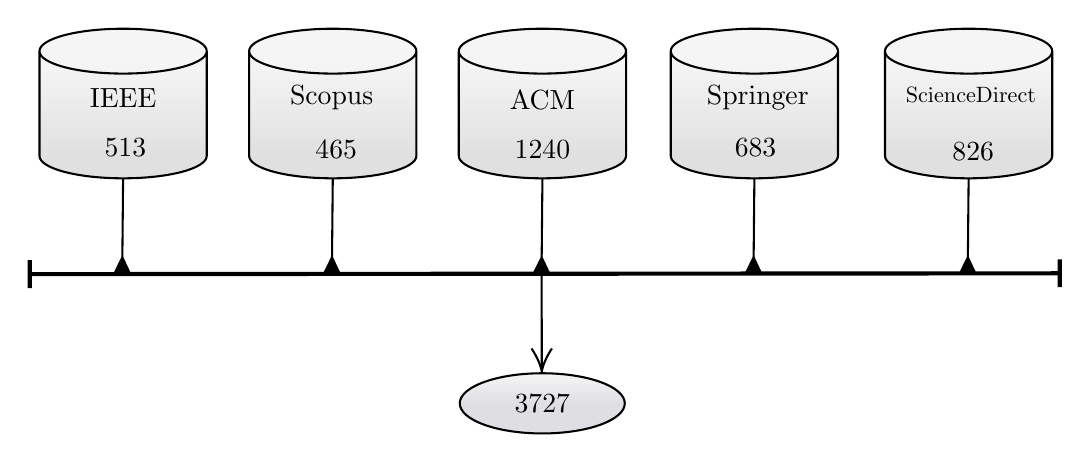
\begin{tikzpicture}[x=0.75pt,y=0.75pt,yscale=-1,xscale=1]
%uncomment if require: \path (0,421); %set diagram left start at 0, and has height of 421

%Shape: Can [id:dp367210882965306] 
\path  [shading=_2uy0ym1vv,_kdbe20a91] (581.45,74.81) -- (581.45,125.27) .. controls (581.45,131.24) and (563.41,136.08) .. (541.16,136.08) .. controls (518.9,136.08) and (500.86,131.24) .. (500.86,125.27) -- (500.86,74.81)(581.45,74.81) .. controls (581.45,80.78) and (563.41,85.62) .. (541.16,85.62) .. controls (518.9,85.62) and (500.86,80.78) .. (500.86,74.81) .. controls (500.86,68.84) and (518.9,64) .. (541.16,64) .. controls (563.41,64) and (581.45,68.84) .. (581.45,74.81) -- cycle ; % for fading 
 \draw   (581.45,74.81) -- (581.45,125.27) .. controls (581.45,131.24) and (563.41,136.08) .. (541.16,136.08) .. controls (518.9,136.08) and (500.86,131.24) .. (500.86,125.27) -- (500.86,74.81)(581.45,74.81) .. controls (581.45,80.78) and (563.41,85.62) .. (541.16,85.62) .. controls (518.9,85.62) and (500.86,80.78) .. (500.86,74.81) .. controls (500.86,68.84) and (518.9,64) .. (541.16,64) .. controls (563.41,64) and (581.45,68.84) .. (581.45,74.81) -- cycle ; % for border 

%Shape: Can [id:dp26297274922570457] 
\path  [shading=_ckay7h6o4,_gma3lvhx6] (478.23,74.81) -- (478.23,125.27) .. controls (478.23,131.24) and (460.19,136.08) .. (437.94,136.08) .. controls (415.68,136.08) and (397.64,131.24) .. (397.64,125.27) -- (397.64,74.81)(478.23,74.81) .. controls (478.23,80.78) and (460.19,85.62) .. (437.94,85.62) .. controls (415.68,85.62) and (397.64,80.78) .. (397.64,74.81) .. controls (397.64,68.84) and (415.68,64) .. (437.94,64) .. controls (460.19,64) and (478.23,68.84) .. (478.23,74.81) -- cycle ; % for fading 
 \draw   (478.23,74.81) -- (478.23,125.27) .. controls (478.23,131.24) and (460.19,136.08) .. (437.94,136.08) .. controls (415.68,136.08) and (397.64,131.24) .. (397.64,125.27) -- (397.64,74.81)(478.23,74.81) .. controls (478.23,80.78) and (460.19,85.62) .. (437.94,85.62) .. controls (415.68,85.62) and (397.64,80.78) .. (397.64,74.81) .. controls (397.64,68.84) and (415.68,64) .. (437.94,64) .. controls (460.19,64) and (478.23,68.84) .. (478.23,74.81) -- cycle ; % for border 

%Shape: Can [id:dp22020354780833284] 
\path  [shading=_a9lyv0hls,_htck7z5md] (376.11,74.81) -- (376.11,125.27) .. controls (376.11,131.24) and (358.07,136.08) .. (335.82,136.08) .. controls (313.56,136.08) and (295.52,131.24) .. (295.52,125.27) -- (295.52,74.81)(376.11,74.81) .. controls (376.11,80.78) and (358.07,85.62) .. (335.82,85.62) .. controls (313.56,85.62) and (295.52,80.78) .. (295.52,74.81) .. controls (295.52,68.84) and (313.56,64) .. (335.82,64) .. controls (358.07,64) and (376.11,68.84) .. (376.11,74.81) -- cycle ; % for fading 
 \draw   (376.11,74.81) -- (376.11,125.27) .. controls (376.11,131.24) and (358.07,136.08) .. (335.82,136.08) .. controls (313.56,136.08) and (295.52,131.24) .. (295.52,125.27) -- (295.52,74.81)(376.11,74.81) .. controls (376.11,80.78) and (358.07,85.62) .. (335.82,85.62) .. controls (313.56,85.62) and (295.52,80.78) .. (295.52,74.81) .. controls (295.52,68.84) and (313.56,64) .. (335.82,64) .. controls (358.07,64) and (376.11,68.84) .. (376.11,74.81) -- cycle ; % for border 

%Shape: Can [id:dp47910417750400036] 
\path  [shading=_e1ldk6rgh,_f0lkgujyf] (275.1,74.81) -- (275.1,125.27) .. controls (275.1,131.24) and (257.06,136.08) .. (234.81,136.08) .. controls (212.55,136.08) and (194.51,131.24) .. (194.51,125.27) -- (194.51,74.81)(275.1,74.81) .. controls (275.1,80.78) and (257.06,85.62) .. (234.81,85.62) .. controls (212.55,85.62) and (194.51,80.78) .. (194.51,74.81) .. controls (194.51,68.84) and (212.55,64) .. (234.81,64) .. controls (257.06,64) and (275.1,68.84) .. (275.1,74.81) -- cycle ; % for fading 
 \draw   (275.1,74.81) -- (275.1,125.27) .. controls (275.1,131.24) and (257.06,136.08) .. (234.81,136.08) .. controls (212.55,136.08) and (194.51,131.24) .. (194.51,125.27) -- (194.51,74.81)(275.1,74.81) .. controls (275.1,80.78) and (257.06,85.62) .. (234.81,85.62) .. controls (212.55,85.62) and (194.51,80.78) .. (194.51,74.81) .. controls (194.51,68.84) and (212.55,64) .. (234.81,64) .. controls (257.06,64) and (275.1,68.84) .. (275.1,74.81) -- cycle ; % for border 

%Shape: Can [id:dp2245173518314696] 
\path  [shading=_7aeqfhyni,_h83ak7psv] (174.09,74.81) -- (174.09,125.27) .. controls (174.09,131.24) and (156.05,136.08) .. (133.79,136.08) .. controls (111.54,136.08) and (93.5,131.24) .. (93.5,125.27) -- (93.5,74.81)(174.09,74.81) .. controls (174.09,80.78) and (156.05,85.62) .. (133.79,85.62) .. controls (111.54,85.62) and (93.5,80.78) .. (93.5,74.81) .. controls (93.5,68.84) and (111.54,64) .. (133.79,64) .. controls (156.05,64) and (174.09,68.84) .. (174.09,74.81) -- cycle ; % for fading 
 \draw   (174.09,74.81) -- (174.09,125.27) .. controls (174.09,131.24) and (156.05,136.08) .. (133.79,136.08) .. controls (111.54,136.08) and (93.5,131.24) .. (93.5,125.27) -- (93.5,74.81)(174.09,74.81) .. controls (174.09,80.78) and (156.05,85.62) .. (133.79,85.62) .. controls (111.54,85.62) and (93.5,80.78) .. (93.5,74.81) .. controls (93.5,68.84) and (111.54,64) .. (133.79,64) .. controls (156.05,64) and (174.09,68.84) .. (174.09,74.81) -- cycle ; % for border 

%Straight Lines [id:da8063181741938354] 
\draw [line width=1.5]    (88.82,182.25) -- (585.07,181.85) ;
\draw [shift={(585.07,181.85)}, rotate = 539.95] [color={rgb, 255:red, 0; green, 0; blue, 0 }  ][line width=1.5]    (0,6.71) -- (0,-6.71)   ;
\draw [shift={(88.82,182.25)}, rotate = 539.95] [color={rgb, 255:red, 0; green, 0; blue, 0 }  ][line width=1.5]    (0,6.71) -- (0,-6.71)   ;
%Straight Lines [id:da04659966611813071] 
\draw    (133.79,136.08) -- (133.43,174.05) ;
\draw [shift={(133.44,173.05)}, rotate = 90.54] [fill={rgb, 255:red, 0; green, 0; blue, 0 }  ][line width=0.75]  [draw opacity=0] (8.93,-4.29) -- (0,0) -- (8.93,4.29) -- cycle    ;

%Straight Lines [id:da7123071533494616] 
\draw [line width=0.75]    (335.45,183.05) -- (335.5,227) ;
\draw [shift={(335.5,229)}, rotate = 269.94] [color={rgb, 255:red, 0; green, 0; blue, 0 }  ][line width=0.75]    (10.93,-4.9) .. controls (6.95,-2.3) and (3.31,-0.67) .. (0,0) .. controls (3.31,0.67) and (6.95,2.3) .. (10.93,4.9)   ;

%Straight Lines [id:da037978733368861706] 
\draw    (234.81,136.08) -- (234.45,174.05) ;
\draw [shift={(234.46,173.05)}, rotate = 90.54] [fill={rgb, 255:red, 0; green, 0; blue, 0 }  ][line width=0.75]  [draw opacity=0] (8.93,-4.29) -- (0,0) -- (8.93,4.29) -- cycle    ;

%Straight Lines [id:da8972295671751513] 
\draw    (335.82,136.08) -- (335.46,174.05) ;
\draw [shift={(335.47,173.05)}, rotate = 90.54] [fill={rgb, 255:red, 0; green, 0; blue, 0 }  ][line width=0.75]  [draw opacity=0] (8.93,-4.29) -- (0,0) -- (8.93,4.29) -- cycle    ;

%Straight Lines [id:da1432985950729515] 
\draw    (437.94,136.08) -- (437.58,174.05) ;
\draw [shift={(437.58,173.05)}, rotate = 90.54] [fill={rgb, 255:red, 0; green, 0; blue, 0 }  ][line width=0.75]  [draw opacity=0] (8.93,-4.29) -- (0,0) -- (8.93,4.29) -- cycle    ;

%Straight Lines [id:da646269410198852] 
\draw    (541.16,136.08) -- (540.8,174.05) ;
\draw [shift={(540.8,173.05)}, rotate = 90.54] [fill={rgb, 255:red, 0; green, 0; blue, 0 }  ][line width=0.75]  [draw opacity=0] (8.93,-4.29) -- (0,0) -- (8.93,4.29) -- cycle    ;

%Shape: Ellipse [id:dp07212159007821795] 
\path  [shading=_o4bxs07nh,_bzbwl9s0d] (296,244.5) .. controls (296,236.49) and (313.8,230) .. (335.75,230) .. controls (357.7,230) and (375.5,236.49) .. (375.5,244.5) .. controls (375.5,252.51) and (357.7,259) .. (335.75,259) .. controls (313.8,259) and (296,252.51) .. (296,244.5) -- cycle ; % for fading 
 \draw   (296,244.5) .. controls (296,236.49) and (313.8,230) .. (335.75,230) .. controls (357.7,230) and (375.5,236.49) .. (375.5,244.5) .. controls (375.5,252.51) and (357.7,259) .. (335.75,259) .. controls (313.8,259) and (296,252.51) .. (296,244.5) -- cycle ; % for border 


% Text Node
\draw (133.79,97.23) node  [align=left] {IEEE};
% Text Node
\draw (234.25,97.23) node  [align=left] {Scopus};
% Text Node
\draw (335.82,98.13) node  [align=left] {ACM};
% Text Node
\draw (439.59,97.13) node  [align=left] {Springer};
% Text Node
\draw (542.26,96.02) node [scale=0.8] [align=left] {ScienceDirect};
% Text Node
\draw (134.9,121.19) node [scale=1] [align=left] {513};
% Text Node
\draw (236.46,122.09) node [scale=1] [align=left] {465};
% Text Node
\draw (335.82,122.09) node [scale=1] [align=left] {1240};
% Text Node
\draw (438.49,121.19) node [scale=1] [align=left] {683};
% Text Node
\draw (543.36,122.98) node [scale=1] [align=left] {826};
% Text Node
\draw (335.75,244.5) node  [align=left] {3727};


\end{tikzpicture}

		\fonte{O autor.}
	\label{fig:ResusltadosBases}
\end{figure}

% \begin{figure}
%     \centering
%     % \includegraphics[scale=0.6]{images/searchprocess.png}
%     \begin{tikzpicture}
%       \begin{scope}[blend group = soft light]
%         \draw[ultra thin, pattern color=gray, pattern=horizontal lines] (90:4.05) circle (2.5);
%         \draw[ultra thin, pattern color=gray, pattern=vertical lines] (90:3.56) circle (2);
%         \draw[ultra thin, pattern color=gray, pattern=crosshatch] (90:3.08) circle (1.5);
%         \draw[ultra thin, fill=gray!45] (90:2.6) circle (1);
%       \end{scope}
%       \node at ( 90:5.9) { \contour{white}{\textbf{633 Retrieved Studies}} };
%       \node at ( 90:4.9) { \contour{white}{\textbf{559 Not duplicates}} };
%       \node at ( 90:4) { \contour{white}{\textbf{52 Included}} };
%       \node at ( 90:2.76) { \contour{white}{\textbf{76 Platforms}} };
%       \node at ( 90:2.46) {\contour{white}{\& \textbf{Providers}} };
%     \end{tikzpicture}
%     \caption{Onion diagram showing the quantity of papers after each step of the SLM process.}
%     \label{fig:searchprocess}
% \end{figure}

\begin{figure}[!htb]
	\centering
	    \caption{Ciclos de seleção dos estudos primários.}
		%\includesvg[width=\textwidth]{img/CiclosDeAvaliacao.svg}
        

% Gradient Info
  
\tikzset {_9ett5n0d2/.code = {\pgfsetadditionalshadetransform{ \pgftransformshift{\pgfpoint{0 bp } { 0 bp }  }  \pgftransformrotate{-90 }  \pgftransformscale{2 }  }}}
\pgfdeclarehorizontalshading{_kkttfrljg}{150bp}{rgb(0bp)=(0.96,0.96,0.96);
rgb(37.5bp)=(0.96,0.96,0.96);
rgb(51.875bp)=(0.87,0.87,0.89);
rgb(100bp)=(0.87,0.87,0.89)}
\tikzset{every picture/.style={line width=0.75pt}} %set default line width to 0.75pt        

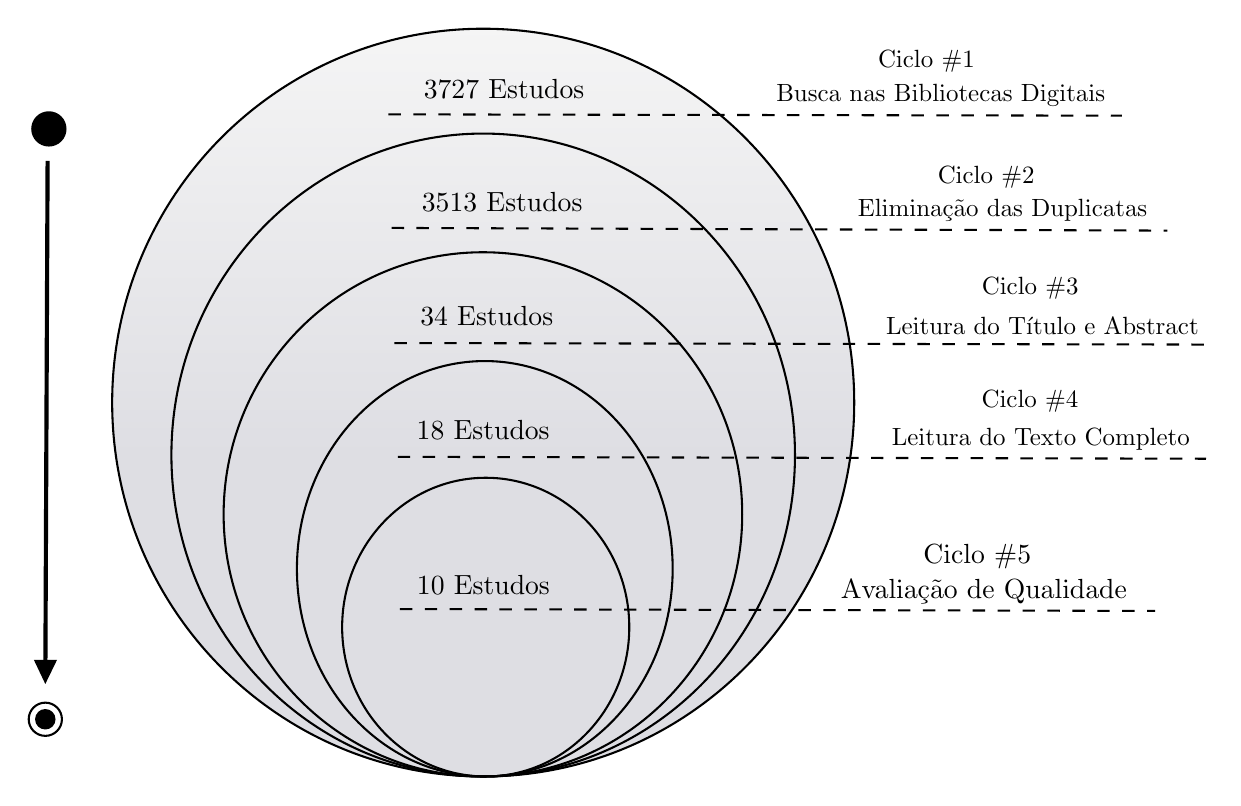
\begin{tikzpicture}[x=0.75pt,y=0.75pt,yscale=-1,xscale=1]
%uncomment if require: \path (0,423); %set diagram left start at 0, and has height of 423

%Flowchart: Connector [id:dp2928546604203144] 
\path  [shading=_kkttfrljg,_9ett5n0d2] (53.5,191.87) .. controls (53.5,92.38) and (133.53,11.73) .. (232.26,11.73) .. controls (330.98,11.73) and (411.02,92.38) .. (411.02,191.87) .. controls (411.02,291.35) and (330.98,372) .. (232.26,372) .. controls (133.53,372) and (53.5,291.35) .. (53.5,191.87) -- cycle ; % for fading 
 \draw   (53.5,191.87) .. controls (53.5,92.38) and (133.53,11.73) .. (232.26,11.73) .. controls (330.98,11.73) and (411.02,92.38) .. (411.02,191.87) .. controls (411.02,291.35) and (330.98,372) .. (232.26,372) .. controls (133.53,372) and (53.5,291.35) .. (53.5,191.87) -- cycle ; % for border 

%Flowchart: Connector [id:dp4856968141430813] 
\draw   (82.04,217.12) .. controls (82.04,131.59) and (149.3,62.25) .. (232.26,62.25) .. controls (315.22,62.25) and (382.47,131.59) .. (382.47,217.12) .. controls (382.47,302.66) and (315.22,372) .. (232.26,372) .. controls (149.3,372) and (82.04,302.66) .. (82.04,217.12) -- cycle ;
%Flowchart: Connector [id:dp8496211285519002] 
\draw   (107.2,245.72) .. controls (107.2,175.97) and (163.13,119.43) .. (232.13,119.43) .. controls (301.12,119.43) and (357.05,175.97) .. (357.05,245.72) .. controls (357.05,315.46) and (301.12,372) .. (232.13,372) .. controls (163.13,372) and (107.2,315.46) .. (107.2,245.72) -- cycle ;
%Flowchart: Connector [id:dp6739952869493944] 
\draw   (142.51,271.93) .. controls (142.51,216.66) and (183.04,171.85) .. (233.03,171.85) .. controls (283.02,171.85) and (323.55,216.66) .. (323.55,271.93) .. controls (323.55,327.2) and (283.02,372) .. (233.03,372) .. controls (183.04,372) and (142.51,327.2) .. (142.51,271.93) -- cycle ;
%Flowchart: Connector [id:dp626524831544014] 
\draw   (164.3,300.04) .. controls (164.3,260.3) and (195.27,228.08) .. (233.47,228.08) .. controls (271.67,228.08) and (302.64,260.3) .. (302.64,300.04) .. controls (302.64,339.78) and (271.67,372) .. (233.47,372) .. controls (195.27,372) and (164.3,339.78) .. (164.3,300.04) -- cycle ;
%Straight Lines [id:da31235038530795767] 
\draw  [dash pattern={on 4.5pt off 4.5pt}]  (186.61,52.99) -- (539.94,53.63) ;


%Straight Lines [id:da5536929778572981] 
\draw  [dash pattern={on 4.5pt off 4.5pt}]  (188.12,107.71) -- (561.94,109) ;


%Straight Lines [id:da6737369833612874] 
\draw  [dash pattern={on 4.5pt off 4.5pt}]  (189.5,163.17) -- (583.25,163.91) ;


%Straight Lines [id:da5470247173512306] 
\draw  [dash pattern={on 4.5pt off 4.5pt}]  (191.11,217.99) -- (580.5,218.91) ;


%Straight Lines [id:da665185906632269] 
\draw  [dash pattern={on 4.5pt off 4.5pt}]  (192.11,291.33) -- (555.98,292.25) ;


%Straight Lines [id:da29299456740910346] 
\draw [line width=1.5]    (22.39,75.43) -- (21.3,324.43) ;
\draw [shift={(21.29,327.43)}, rotate = 270.25] [fill={rgb, 255:red, 0; green, 0; blue, 0 }  ][line width=1.5]  [draw opacity=0] (11.61,-5.58) -- (0,0) -- (11.61,5.58) -- cycle    ;

%Flowchart: Connector [id:dp48946546663936763] 
\draw  [fill={rgb, 255:red, 0; green, 0; blue, 0 }  ,fill opacity=1 ] (15,60) .. controls (15,55.58) and (18.58,52) .. (23,52) .. controls (27.42,52) and (31,55.58) .. (31,60) .. controls (31,64.42) and (27.42,68) .. (23,68) .. controls (18.58,68) and (15,64.42) .. (15,60) -- cycle ;
%Flowchart: Connector [id:dp24133340263386382] 
\draw   (13.29,344.43) .. controls (13.29,340.01) and (16.87,336.43) .. (21.29,336.43) .. controls (25.7,336.43) and (29.29,340.01) .. (29.29,344.43) .. controls (29.29,348.85) and (25.7,352.43) .. (21.29,352.43) .. controls (16.87,352.43) and (13.29,348.85) .. (13.29,344.43) -- cycle ;
%Flowchart: Connector [id:dp2687972500754565] 
\draw  [fill={rgb, 255:red, 0; green, 0; blue, 0 }  ,fill opacity=1 ] (16.87,344.43) .. controls (16.87,341.99) and (18.85,340.01) .. (21.29,340.01) .. controls (23.72,340.01) and (25.7,341.99) .. (25.7,344.43) .. controls (25.7,346.87) and (23.72,348.85) .. (21.29,348.85) .. controls (18.85,348.85) and (16.87,346.87) .. (16.87,344.43) -- cycle ;

% Text Node
\draw (445.81,27.26) node [scale=0.9] [align=left] {Ciclo \#1};
% Text Node
\draw (452.7,43.84) node [scale=0.9] [align=left] {Busca nas Bibliotecas Digitais};
% Text Node
\draw (474.6,83.22) node [scale=0.9] [align=left] {Ciclo \#2};
% Text Node
\draw (495.84,136.68) node [scale=0.9] [align=left] {Ciclo \#3};
% Text Node
\draw (495.72,191.35) node [scale=0.9] [align=left] {Ciclo \#4};
% Text Node
\draw (470.32,265.86) node [scale=1] [align=left] {Ciclo \#5};
% Text Node
\draw (242.31,40.79) node [scale=1] [align=left] {3727 Estudos};
% Text Node
\draw (482.49,99.04) node [scale=0.9] [align=left] {Eliminação das Duplicatas};
% Text Node
\draw (241.4,94.97) node [scale=1] [align=left] {3513 Estudos};
% Text Node
\draw (501.67,155.11) node [scale=0.9] [align=left] {Leitura do Título e Abstract};
% Text Node
\draw (233.99,150.1) node [scale=1] [align=left] {34 Estudos};
% Text Node
\draw (500.9,209.51) node [scale=0.9] [align=left] {Leitura do Texto Completo};
% Text Node
\draw (232.26,205.21) node [scale=1] [align=left] {18 Estudos};
% Text Node
\draw (473.47,282.92) node [scale=1] [align=left] {Avaliação de Qualidade};
% Text Node
\draw (232.38,279.6) node [scale=1] [align=left] {10 Estudos};


\end{tikzpicture}

		\fonte{O autor.}
	\label{fig:CiclosRevisao}
\end{figure}

Com o conjunto inicial de 3727 estudos primários identificados, 
%os ciclos de seleção foram iniciados, totalizando cinco (5).
foram definidos cinco (5) ciclos de seleção, apresentados na \autoref{fig:CiclosRevisao}. 
Nestas iterações houve a exclusão de estudos duplicados (restando 3513), a seleção de estudos baseado em título e \textit{abstract} (restando 34), seleção baseada em texto completo (restando 18) e a seleção baseada na avaliação de qualidade (restando 10). 
Cada iteração tinha o objetivo de eliminar estudos que estavam fora do escopo da pesquisa ou considerados não relevantes. 
Na última iteração, 18 estudos tiveram sua qualidade analisada. 
Foi estabelecido que apenas estudos com pontuação acima de 5 (cinco) seriam aceitos. 
Assim, após a aplicação dos \ac{CQ} foram excluídos 8 (oito) trabalhos. 
O conjunto final de dez (10) estudos aprovados na \ac{SLM} seguiu para a etapa de extração de dados. 
Entre estes trabalhos a menor pontuação foi de 5.3, enquanto o maior alcançou 10. 
A \autoref{tab:AvalQualidade} resume os resultados obtidos na avaliação da qualidade. 

A execução do protocolo de busca na \textit{grey literature} retornou um total de 132 ferramentas. 
Após sumarização foi realizado a exclusão de duplicatas (restando 67).
%, e chegou-se a um número final de 67 ferramentas. 
Durante esse processo houve doze (12) ferramentas que não puderam ser avaliadas 
% por algum tipo indisponibilidade, 
\textit{e.g.} impossibilidade de instalação ou incompatibilidade com o ambiente utilizado. 
Ao fim, foi possível executar testes de uso com um total de 55 ferramentas, e consequentemente, a extração dos dados relevantes ao estudo. 
Durante o uso das ferramentas foram realizados modelos simples de \acp{BD}, em que se procurou observar o suporte aos níveis de modelagem e as notações e linguagens usadas.

%#################################################################
\section{Resultados e Discussão} \label{sec:ResultDis}
%#################################################################

Os estudos primários foram avaliados com base nos critérios de qualidade definidos na \autoref{scec:AvalQualidade}.
A menor pontuação foi de 5,3 enquanto o maior alcançou 10. 
A \autoref{tab:AvalQualidade} resume os resultados obtidos na avaliação da qualidade.

\rowcolors{1}{gray!15}{white}
\begin{table}[!htb]
\footnotesize
\centering
\caption{Resultados da avaliação de qualidade.}
\label{tab:AvalQualidade}
\begin{tabular}{lcccccccr}
\bottomrule
\rowcolor[HTML]{C0C0C0}
\multicolumn{1}{c}{\textbf{Estudos}} &
\multicolumn{7}{c}{\textbf{Critérios de Qualidade}} &
\multicolumn{1}{r}{\textbf{Pontuação}} \\
\hline
\rowcolor[HTML]{C0C0C0}\textbf{Referência} & 
\textbf{CQ1} & \textbf{CQ2} & \textbf{CQ3} & \textbf{CQ4} & \textbf{CQ5} & \textbf{CQ6} & \textbf{CQ7} & 
\textbf{Total} \\
\hline
\citeonline{Ayadi:2016} & 
P & P & T & P & N & T & P &
5,7 \\
\citeonline{Celikovic:2014} & 
T & T & N & T & P & P & T &
7,0 \\
\citeonline{Dimitrieski:2015} & 
T & T & T & T & T & T & T &
10,0
\\
\citeonline{Hammer:1981} & 
T & T & N & T & N & P & P &
5,5 \\
\citeonline{Jagannathan:1988} & 
T & T & N & T & P & N & N &
5,5 \\
\citeonline{Kersten:2011} & 
P & T & T & P & N & N & P &
5,3 \\
\citeonline{Litwin:1989} & 
P & T & N & T & N & P & T &
5,4 \\
\citeonline{Mazairac:2013} & 
T & T & P & T & N & N & P &
5,9 \\
\citeonline{Shipman:1981} & 
T & T & N & T & P & N & P &
6,0 \\
\citeonline{Tian:2006} & 
T & P & N & T & P & P & T &
6,4 \\
%\hline
%\citeonline{Vagner:2018} & 
%T & T & P & N & N & P & P &
%4.9 \\
%\citeonline{Bogdanova:2019} & 
%T & P & P & N & N & T & P &
%4.8 \\
%\citeonline{Ribic:2018} & 
%N & N & T & T & N & P & T &
%4.5 \\
%\citeonline{Morgan:2018} & 
%N & N & T & N & N & P & P &
%2.5 \\
%\citeonline{Karakonda:1990} & 
%P & P & N & N & N & N & N &
%1.8 \\
%\citeonline{Zhang:2016} & 
%N & N & N & N & N & P & T &
%1.5 \\
%\citeonline{Schuler:2018} & 
%N & N & N & N & N & P & P &
%1.0 \\
\hline
\end{tabular}
\fonte{O autor.}
\end{table}

Em relação ao estado da arte (\textbf{QP1}) do desenvolvimento de \ac{DSL} aplicado na transformação de modelos de dados, identificou-se um estudo que apresenta a \textit{System Modeling Tool} (MIST), o qual utiliza uma \ac{DSL} bidirecional para modelagem conceitual de \acp{BD}, chamado \textit{EERDSL}. 

Quanto às metodologias, técnicas ou propostas de refinamento (\textbf{QP1.1}) baseadas em modelos de dados, apenas os dois estudos mencionados aplicam conceitos para refinamento, sendo que tais conceitos são apoiados na normalização de \acp{BD} para auxiliar os desenvolvedores que utilizam sua solução.

No que se refere às tecnologias usadas como suporte para o desenvolvimento de \acp{DSL} (\textbf{QP1.2}), foram registradas Xtext, Xtend, Sirius e Eugenia \cite{Celikovic:2014, Dimitrieski:2015}, StarUML \cite{Ayadi:2016}, IfcDoc Tool e ViewEdit Tool \cite{Mazairac:2013}, MonetDB \cite {Kersten:2011}, Java, JFlex e JCup \cite{Tian:2006}. 
No entanto, estudos mais antigos eram geralmente especificações de \acp{DSL}, não apresentando qualquer forma de implementação ou ferramenta usada \cite{Shipman:1981, Jagannathan:1988, Litwin:1989}.

As representações de \ac{BD} adotadas (\textbf{QP1.3}) possuem \texttt{Tables} e \texttt{Functions} em todos os estudos primários analisados.
Há também referências explícitas à definição de \texttt{Stored Procedures}, \texttt{Triggers} e \texttt{Views} em outros estudos. 
A \autoref{tab:Obj_DSL} resume esses dados recuperados de cada um dos estudos primários. 
Quanto ao uso de \ac{DSL} para transformação de modelos de dados em casos reais (\textbf{QP2}, \textbf{RQ2.1}), nenhuma referência foi encontrada nos estudos avaliados.

\rowcolors{1}{gray!15}{white}
\begin{table}[!htb]
    \centering
    \scriptsize
    \caption{Objetos de banco de dados representados.}
    \label{tab:Obj_DSL}
    \begin{tabular}{llccccc}
    \bottomrule
    \rowcolor[HTML]{C0C0C0}
    \multicolumn{2}{c}{\textbf{Estudo Primário}} &
    \multicolumn{5}{c}{\textbf{Objetos de BD}} \\
    \hline
    \rowcolor[HTML]{C0C0C0}
    \textbf{Referência} & \textbf{DSL} &
    \textbf{Tables} & \textbf{SP} & \textbf{Functions} & \textbf{Triggers} &\textbf{Views}\\
    \hline
    \citeonline{Ayadi:2016} & Ayadi's Notation & 
    \checkmark & & & & \\
    \citeonline{Celikovic:2014} & EERDSL v.1 &
    \checkmark & & \checkmark & \checkmark & \\
    \citeonline{Dimitrieski:2015} & EERDSL v.2 & 
    \checkmark & \checkmark & \checkmark & \checkmark & \checkmark \\
    \citeonline{Hammer:1981} & SDM &
    \checkmark & & & \checkmark & \\
    \citeonline{Jagannathan:1988}   & SDM &
    \checkmark & & \checkmark & & \\
    \citeonline{Kersten:2011}& SciSQL &
    \checkmark & & \checkmark & & \\
    \citeonline{Litwin:1989} & MSQL &
    \checkmark & \checkmark & \checkmark & \checkmark & \checkmark \\
    \citeonline{Mazairac:2013} & BIMQL &
    \checkmark & \checkmark & \checkmark & & \\
    \citeonline{Shipman:1981} & DAPLEX &
    \checkmark & & \checkmark & & \\
    \citeonline{Tian:2006} & NeuroQL & 
    \checkmark & & \checkmark & & \\
    \toprule
    \end{tabular}
    \\
    \textbf{Legenda}: SP = \textit{Stored Procedures}.
    \\
    \fonte{O autor.}
\end{table}

Sobre os métodos usados para avaliar as \acp{DSL} (\textbf{QP2.2}) existe apenas um estudo preliminar que apresenta a validação da proposta \cite{Dimitrieski:2015} usando dezesseis (16) participantes, sendo dois (2) especialistas em \ac{IHC}, três (3) especialistas em modelagem de sistemas e onze (11) estudantes. Entre os estudantes seis (6) eram mestrandos na área de \acp{BD} e cinco (5) doutorandos com experiência em modelagem.
Em geral, os outros estudos indicam a falta de uma avaliação de suas proposições como um possível trabalho futuro.

Entre os aspectos positivos e negativos observados (\textbf{RQ2.3}) nos estudos, houve observações favoráveis à facilidade de compreensão, a modelagem intuitiva e independência de plataformas específicas \cite{Tian:2006, Mazairac:2013}.
Pontos negativos foram a falta de geração automática de \ac{SQL} para sistemas de \ac{BD} \cite{Ayadi:2016} ou uma limitação neste item \cite{Dimitrieski:2015}.
Ainda há um registro da falta de implementação real de \acp{DSL} até o momento em que o estudo foi realizado, havendo apenas especificações \cite{Hammer:1981, Jagannathan:1988, Tian:2006, Kersten:2011, Ayadi:2016}.
Os principais desafios identificados pelos estudos (\textbf{RQ2.4}), em geral, são as avaliações das abordagens, bem como a evolução e/ou simplificação das propostas.
Finalmente, na \autoref{tab:DSL_type} as \acp{DSL} são apresentadas em relação ao seu tipo.
No entanto, é importante observar que os estudos que marcam a coluna \texttt{bidirecional} \cite{Celikovic:2014, Dimitrieski:2015} são versões diferentes da mesma implementação de \ac{DSL}, enquanto o \cite{Hammer:1981, Jagannathan:1988} são uma especificação de \ac{DSL} e implementação com base nesta especificação, respectivamente.

\rowcolors{1}{gray!15}{white}
\begin{table}[!htb]
    \centering
    \footnotesize
    \caption{Categorização das DSLs propostas.}
    \label{tab:DSL_type}
    \begin{tabular}{llccc}
    \bottomrule
    \rowcolor[HTML]{C0C0C0}
    \multicolumn{2}{c}{\textbf{Estudos Primários}} &
    \multicolumn{3}{c}{\textbf{Tipo de DSL}} \\
    \hline
    \rowcolor[HTML]{C0C0C0}
    \textbf{Referência} & \textbf{DSL} & 
    \textbf{Textual} & \textbf{Gráfica} & \textbf{Bidirecional} \\
    \hline
    \citeonline{Ayadi:2016} & Ayadi's Notation & & \checkmark & \\
    \citeonline{Celikovic:2014} & EERDSL v.1 & & &\checkmark \\
    \citeonline{Dimitrieski:2015} & EERDSL v.2 & & & \checkmark\\
    \citeonline{Hammer:1981} & SDM & \checkmark & & \\
    \citeonline{Jagannathan:1988} & SDM & \checkmark & & \\
    \citeonline{Kersten:2011} & SciQL & \checkmark & & \\
    \citeonline{Litwin:1989} & MSQL & \checkmark & & \\
    \citeonline{Mazairac:2013} & BIMQL & \checkmark & & \\
    \citeonline{Shipman:1981} & DAPLEX & \checkmark & & \\
    \citeonline{Tian:2006} & NeuroQL & \checkmark & & \\
    \toprule
    \end{tabular}
    \fonte{O autor.}
\end{table}

Quanto ao estado da prática (\textbf{QP3}) das ferramentas utilizadas na modelagem de \ac{BD}, foram mapeadas 55 ferramentas. 
Houve a classificação quanto ao seu tipo, sendo 29 exclusivas de modelagem \ac{BD} (\textit{Data Modeling}), 13 de modelagem que ainda oferecem conexão com \ac{BD} e execução de consultas (\textit{Full IDE}), 10 com suporte a diagramação de diversos tipos de modelos (\textit{Diagramming}) e 3 ferramentas projetadas para grandes empresas, podendo diagramar inúmeros tipos de documentos e processos (\textit{Enterprise Modeling}). 

Em relação às notações utilizadas nas ferramentas (\textbf{QP3.1}) foram identificados mais de 10 (dez) variedades de notações, com destaque a notação \textit{Crow's Foot} com 35 ocorrências e da notação IDEF1X com 23 registros. 
Esses e outros dados estão listados nas Tabelas \ref{tab:ResultsI} e \ref{tab:ResultsII}.

Finalmente, no que diz respeito aos modelos suportados pelas ferramentas (\textbf{QP3.2}) foi constatado que individualmente 26 ferramentas oferecem suporte a modelagem conceitual, 48 ferramentas à modelagem lógica e 37 à modelagem física. 
O conjunto representando as intersecções do suporte aos modelos quanto às ferramentas é exibido na \autoref{fig:VennDiagram}.

\rowcolors{0}{}{}
\begin{figure}[!htb]
\centering
\caption{Diagrama de Venn dos modelos suportados nas ferramentas.}
%\rowcolors{0}{}{}
%\begin{figure}[!htb]
\centering
\def\firstcircle{(-3, 1.5) circle (3.5)} % Lógico
\def\secondcircle{(-0.5, 1.5) circle (3)} % Físico
\def\thirdcircle{(-2.3, -1.5) circle (2.5)} % Conceitual
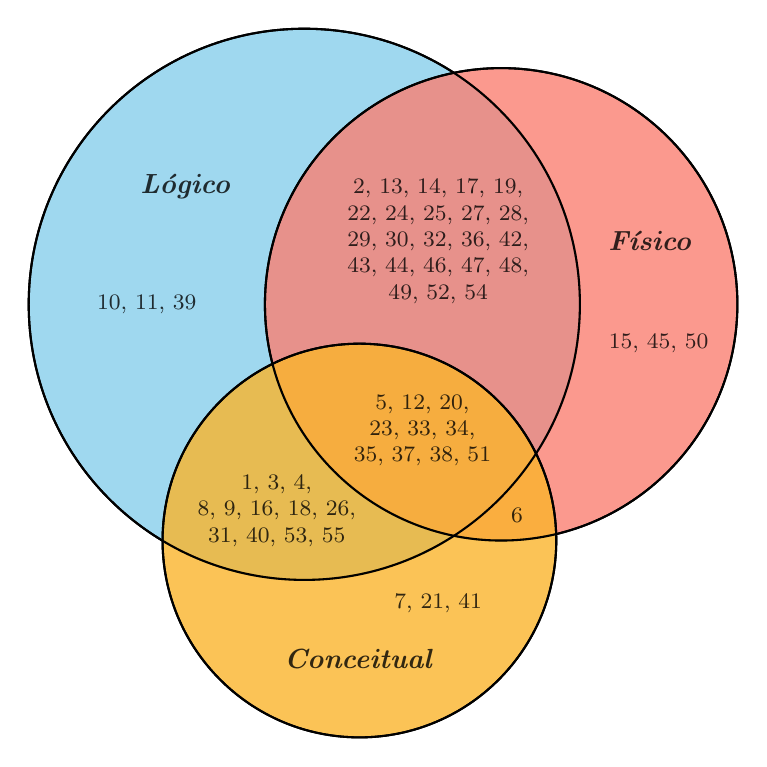
\begin{tikzpicture}
\centering
\begin{scope}[shift={(4cm,-15cm)}, fill opacity=.8]
        \fill[SkyBlue, draw = black] \firstcircle;
        \fill[Salmon, draw = black] \secondcircle;
        \fill[Dandelion, draw = black] \thirdcircle;
        \draw \firstcircle node at(-1.3, -2.3) {
        \footnotesize
        \begin{tabular}{c}
        %\textbf{CONCEITUAL} \\ %Conceitual
         7, 21, 41
        \end{tabular}
        };
        \draw \secondcircle  node at(-5, 1.5) %[text width=5cm,align=center] 
        {
        \footnotesize
        \begin{tabular}{c}
        %\textbf{LÓGICO} \\ %Lógico
        10, 11, 39
        \end{tabular}
        };
        \draw \thirdcircle node at(1.5, 1) %[text width=2.7cm,align=center] 
        {
        \footnotesize
        \begin{tabular}{c}
        %\textbf{FÍSICO}\\ %Físico
        15, 45, 50
        \end{tabular}
        };
        \draw node at(-3.35 ,-1.12) { 
        \footnotesize
        \begin{tabular}{c} 
        %Conceitual + Lógico
        1, 3, 4,\\
        8, 9, 16, 18, 26,\\
        31, 40, 53, 55
        \end{tabular}
        };
        \draw node at(-1.5, -0.1) { 
        \footnotesize
        \begin{tabular}{c} 
        %Conceitual + Lógico + Físico
        5, 12, 20,\\
        23, 33, 34,\\
        35, 37, 38, 51
        \end{tabular}
        };
        \draw node at(-1.3, 2.3) { 
        \footnotesize
        \begin{tabular}{c} 
        %Lógico + Físico
        2, 13, 14, 17, 19,\\
        22, 24, 25, 27, 28,\\
        29, 30, 32, 36, 42,\\
        43, 44, 46, 47, 48,\\
        49, 52, 54
        \end{tabular}
        };
        \draw node at(-0.3, -1.2) { 
        \footnotesize
        \begin{tabular}{c} 
        %Conceitual + Físico
        6
        \end{tabular}
        };
        
    \node at (-4.5,3) {\textit{\textbf{Lógico}}};
    \node at (1.4,2.3) {\textit{\textbf{Físico}}};
    \node at (-2.3,-3) {\textit{\textbf{Conceitual}}};
    
    %\begin{scope} %Código para as interseções
    %    \clip \firstcircle;
    %    \fill[lightgray] \secondcircle;
    %\end{scope}
    
    \end{scope}
\end{tikzpicture}
%\caption{Diagrama de Venn dos modelos suportados nas ferramentas.}
%\label{fig:VennDiagram}
%\end{figure}
\fonte{O autor.}
\label{fig:VennDiagram}
\end{figure}

\rowcolors{1}{gray!15}{white}

\begin{landscape}
\begin{table}
    \caption{Ferramentas para modelagem de bancos de dados.}
    \label{tab:ResultsI}
    \centering
    \tiny
    
    \begin{tabular}{l|l|cccc|ccc|cccccccc|cc|cc}
    \bottomrule
    \rowcolor[HTML]{C0C0C0}
    \multicolumn{2}{l}{} &
    \multicolumn{4}{c}{\textbf{Tipo}} &
    \multicolumn{3}{c}{\textbf{Modelos}} &
    \multicolumn{8}{c}{\textbf{Notações Suportadas}} &
    \multicolumn{2}{c}{\textbf{Ambiente}} &
    \multicolumn{2}{c}{\textbf{Licença}}
    \\ 
    \hline
    \rowcolor[HTML]{C0C0C0}
    \# & \textbf{Ferramenta} &
    \textbf{DM} & \textbf{FIDE} & \textbf{DG} & \textbf{EM} &
    \textbf{C} & \textbf{L} & \textbf{F} &
    \textbf{CF} & \textbf{IDEF1x} & \textbf{CN} & \textbf{MN} & \textbf{UML} & \textbf{BN} & \textbf{AN} & \textbf{ON} & 
    \textbf{D} &\textbf{W} &  
    \textbf{C} &\textbf{G}
    \\
1 & AnalyseSI	&	\checkmark	&&&	&	\checkmark	&	\checkmark	&&&	\checkmark	&&	\checkmark	&&&&	&	\checkmark	&	&&	\checkmark\\
2 & Aqua Data Studio ER Modeler	&&	\checkmark	&&	&&	\checkmark	&	\checkmark	&	\checkmark	&	\checkmark	&&&&&&	&	\checkmark	&	&	\checkmark	&	\\
3 & Astah	&&&	\checkmark	&	&	\checkmark	&	\checkmark	&&	\checkmark	&	\checkmark	&&&&&&	&	\checkmark	&	&	\checkmark	&	\\
4 & brModelo	&&&	\checkmark	&	&	\checkmark	&	\checkmark	&&&	\checkmark	&	\checkmark	&&&&	&	\checkmark	&	&&	\checkmark\\
5 & Creately	&&&	\checkmark	&	&	\checkmark	&	\checkmark	&&	\checkmark	&&&&&&&	&&	\checkmark&	\checkmark	&	\\
6 & Database Deployment Manager	&&	\checkmark	&&	&	\checkmark	&	\checkmark	&	\checkmark	&&&	\checkmark	&&&&&	&	\checkmark	&	&&	\checkmark\\
7 & Database Workbench	&&	\checkmark	&&	&	\checkmark	&&	\checkmark	&	\checkmark	&&&&&&&	&	\checkmark	&	&	\checkmark	&	\\
8 & DB Designer	&	\checkmark	&&&	&	\checkmark	&&&&&&&&&&	\checkmark&	\checkmark	&	&	\checkmark	&	\\
9 & DB-Main	&	\checkmark	&&&	&	\checkmark	&	\checkmark	&&&&&&	\checkmark	&&&	&	\checkmark	&	&&	\checkmark\\
10 & DBDesigner 4	&	\checkmark	&&&	&	\checkmark	&	\checkmark	&&	\checkmark	&	\checkmark	&&	\checkmark	&&&&	&	\checkmark	&	&&	\checkmark\\
11 & DBDesigner.net	&	\checkmark	&&&	&&	\checkmark	&&&&&&&&&	\checkmark&&	\checkmark&	\checkmark	&	\\
12 & dbdiagram.io	&	\checkmark	&&&	&&	\checkmark	&&&&&&&&&	\checkmark&&	\checkmark&&	\checkmark\\
13 & dbDiffo	&	\checkmark	&&&	&	\checkmark	&	\checkmark	&	\checkmark	&	\checkmark	&&&&&&	\checkmark	&	&&	\checkmark&&	\checkmark\\
14 & dbForge Studio for MySQL	&&	\checkmark	&&	&&	\checkmark	&	\checkmark	&	\checkmark	&	\checkmark	&&&&&&	&	\checkmark	&	&	\checkmark	&	\\
15 & DBSchema	&&	\checkmark	&&	&&	\checkmark	&	\checkmark	&	\checkmark	&	\checkmark	&&&&	\checkmark	&&	&	\checkmark	&	&	\checkmark	&	\\
16 & DBVisualizer	&&	\checkmark	&&	&&&	\checkmark	&&&&&&&&	\checkmark&	\checkmark	&	&	\checkmark	&	\\
17 & DbWrench	&	\checkmark	&&&	&	\checkmark	&	\checkmark	&&	\checkmark	&&&&&&&	&	\checkmark	&	&	\checkmark	&	\\
18 & DeZign for Databases	&	\checkmark	&&&	&&	\checkmark	&	\checkmark	&	\checkmark	&	\checkmark	&&&&&&	&	\checkmark	&	&	\checkmark	&	\\
19 & Dia	&&&	\checkmark	&	&	\checkmark	&	\checkmark	&&	\checkmark	&	\checkmark	&	\checkmark	&&	\checkmark	&	\checkmark	&	\checkmark	&	&	\checkmark	&	&&	\checkmark\\
20 & dModelAid	&	\checkmark	&&&	&&	\checkmark	&	\checkmark	&&&&&&&&	&&	\checkmark&	\checkmark	&	\\
21 & Enterprise Architect	&&&&	\checkmark&	\checkmark	&	\checkmark	&	\checkmark	&	\checkmark	&	\checkmark	&&&&&&	&	\checkmark	&	&	\checkmark	&	\\
22 & ER-Assistant	&	\checkmark	&&&	&	\checkmark	&&&	\checkmark	&&&&&&&	&	\checkmark	&	&&	\checkmark\\
23 & ER/Builder	&	\checkmark	&&&	&&	\checkmark	&	\checkmark	&&&&&&&&	\checkmark&	\checkmark	&	&&	\checkmark\\
24 & ER/Studio Data Architect	&	\checkmark	&&&	&	\checkmark	&	\checkmark	&	\checkmark	&	\checkmark	&	\checkmark	&&&&&&	&	\checkmark	&	&	\checkmark	&	\\
25 & ERD Concepts	&&	\checkmark	&&	&&	\checkmark	&	\checkmark	&	\checkmark	&	\checkmark	&&&&&&	&	\checkmark	&	&	\checkmark	&	\\
26 & ERDesigner NG	&	\checkmark	&&&	&&	\checkmark	&	\checkmark	&	\checkmark	&&&&&&&	&	\checkmark	&	&&	\checkmark\\
27 & ERDPlus	&	\checkmark	&&&	&	\checkmark	&	\checkmark	&&	\checkmark	&&&&&&&	&&	\checkmark&&	\checkmark\\
28 & Erwin Data Modeler	&	\checkmark	&&&	&&	\checkmark	&	\checkmark	&	\checkmark	&	\checkmark	&&&&&&	&	\checkmark	&	&	\checkmark	&	\\
    \toprule
    \end{tabular}
    \begin{tablenotes}
    \tiny
    \item Legenda: DM (\textit{Data Modeling}) FIDE (\textit{Full IDE}) DG (\textit{Diagramming}) EM (\textit{Enterprise Modeling}) | 
    C (Conceitual) L (Lógico) F (Físico) | 
    CF (\textit{Crow's Foot}) CN (\textit{Chen's Notation}) 
    \item MN (\textit{Merise Notation}) BN (\textit{Barker's Notation}) AN (\textit{Arrow Notation}) ON (\textit{Other Notation}) | 
    D (\textit{Desktop}) W (Web) C (Comercial) G (\textit{Gratu\'ita})
    \end{tablenotes}
    \fonte{O autor.}
\end{table}
\end{landscape}


\rowcolors{1}{gray!15}{white}
\begin{landscape}
    \begin{table}
    \centering
    \tiny
    \caption{Ferramentas para modelagem de bancos de dados (continuação).}    
    \label{tab:ResultsII}
    \begin{tabular}{l|l|cccc|ccc|cccccccc|cc|cc}
    \bottomrule
    \rowcolor[HTML]{C0C0C0}
    \multicolumn{2}{l}{} &
    \multicolumn{4}{c}{\textbf{Tipo}} &
    \multicolumn{3}{c}{\textbf{Modelos}} &
    \multicolumn{8}{c}{\textbf{Notações Suportadas}} &
    \multicolumn{2}{c}{\textbf{Ambiente}} &
    \multicolumn{2}{c}{\textbf{Licença}}
    \\ 
    \hline
    \rowcolor[HTML]{C0C0C0}
    \# & \textbf{Ferramenta} &
    \textbf{DM} & \textbf{FIDE} & \textbf{DG} & \textbf{EM} &
    \textbf{C} & \textbf{L} & \textbf{F} &
    \textbf{CF} & \textbf{IDEF1x} & \textbf{CN} & \textbf{MN} & \textbf{UML} & \textbf{BN} & \textbf{AN} & \textbf{ON} & 
    \textbf{D} &\textbf{W} &  
    \textbf{C} &\textbf{G}
\\
29 & GenMyModel RDS	&&&	\checkmark	&	&&	\checkmark	&	\checkmark	&	\checkmark	&&&&&&&	&&	\checkmark&	\checkmark	&	\\
30 & InfoSphere Data Architect	&&&&	\checkmark&&	\checkmark	&	\checkmark	&	\checkmark	&	\checkmark	&&&&&&	&	\checkmark	&	&	\checkmark	&	\\
31 & Jeddict	&&&	\checkmark	&	&&	\checkmark	&	\checkmark	&	\checkmark	&&&&&&&	&	\checkmark	&	&&	\checkmark\\
32 & ModelRight	&	\checkmark	&&&	&	\checkmark	&	\checkmark	&&&	\checkmark	&&&&&&	&	\checkmark	&	&	\checkmark	&	\\
33 & MySQL Workbench	&&	\checkmark	&&	&&	\checkmark	&	\checkmark	&	\checkmark	&	\checkmark	&&&	\checkmark	&&&	\checkmark&	\checkmark	&	&&	\checkmark\\
34 & Navicat Data Modeler	&	\checkmark	&&&	&	\checkmark	&	\checkmark	&	\checkmark	&	\checkmark	&	\checkmark	&&&&&&	&	\checkmark	&	&	\checkmark	&	\\
35 & Navicat Data Modeler	&	\checkmark	&&&	&	\checkmark	&	\checkmark	&	\checkmark	&	\checkmark	&	\checkmark	&&&	\checkmark	&&&	&	\checkmark	&	&	\checkmark	&	\\
36 & Open ModelSphere	&	\checkmark	&&&	&	\checkmark	&	\checkmark	&	\checkmark	&	\checkmark	&&	\checkmark	&	\checkmark	&&&&	&	\checkmark	&	&&	\checkmark\\
37 & Oracle SQL Developer Data Modeler	&&	\checkmark	&&	&&	\checkmark	&	\checkmark	& \checkmark & \checkmark &&&&&&	&	\checkmark	&	&&	\checkmark\\
38 & pgModeler	&	\checkmark	&&&	&\checkmark&\checkmark&\checkmark&&&&&&&&	\checkmark&	\checkmark	&	&&	\checkmark\\
39 & PowerDesigner	&&&&	\checkmark&	\checkmark	&	\checkmark	&	\checkmark	&	\checkmark	&	\checkmark	&	\checkmark	&	\checkmark	&&	\checkmark	&&	&	\checkmark	&	&	\checkmark	&	\\
40 & QuickDBD	&	\checkmark	&&&	&&	\checkmark	&&&&&&&&&	\checkmark&&	\checkmark&	\checkmark	&	\\
41 & RISE	&&&	\checkmark	&	&	\checkmark	&	\checkmark	&&	\checkmark	&&&&&&&	&	\checkmark	&	&&	\checkmark\\
42 & Software Ideas Modeler	&&&	\checkmark	&	&	\checkmark	&&&	\checkmark	&	\checkmark	&	\checkmark	&&&&&	&	\checkmark	&	&	\checkmark	&	\\
43 & SQL Database Modeler	&	\checkmark	&&&	&&	\checkmark	&	\checkmark	&&	\checkmark	&&&&&&	&&	\checkmark&	\checkmark	&	\\
44 & SQL Maestro	&&	\checkmark	&&	&&	\checkmark	&	\checkmark	&&	\checkmark	&&&&&&	&	\checkmark	&	&	\checkmark	&	\\
45 & SQL Power Architect	&	\checkmark	&&&	&&	\checkmark	&	\checkmark	&	\checkmark	&&&&&&&	&	\checkmark	&	&	\checkmark	&	\\
46 & SQL Server Management Studio	&&	\checkmark	&&	&&&	\checkmark	&&&&&&&&	\checkmark&	\checkmark	&	&&	\checkmark\\
47 & SQLDBM	&	\checkmark	&&&	&&	\checkmark	&	\checkmark	&&	\checkmark	&&&&&&	&&	\checkmark&&	\checkmark\\
48 & SQLyog	&&	\checkmark	&&	&&	\checkmark	&	\checkmark	&&&&&&&&	\checkmark&	\checkmark	&	&	\checkmark	&	\\
49 & Toad Data Modeler	&	\checkmark	&&&	&&	\checkmark	&	\checkmark	&	\checkmark	&	\checkmark	&&&&&&	&	\checkmark	&	&	\checkmark	&	\\
50 & Valentina Studio	&&	\checkmark	&&	&&	\checkmark	&	\checkmark	&	\checkmark	&&&&&&&	&	\checkmark	&	&	\checkmark	&	\\
51 & Vertabelo	&	\checkmark	&&&	&&&	\checkmark	&	\checkmark	&&&&&&&	&&	\checkmark&	\checkmark	&	\\
52 & Visual Paradigm	&&&	\checkmark	&	&	\checkmark	&	\checkmark	&	\checkmark	&	\checkmark	&&&&&&&	&	\checkmark	&	&	\checkmark	&	\\
53 & Win A\&D	&&&	\checkmark	&	&&	\checkmark	&	\checkmark	&	\checkmark	&&&&&&&	&	\checkmark	&	&	\checkmark	&	\\
54 & WWW SQL Designer	&	\checkmark	&&&	&	\checkmark	&	\checkmark	&&&&&&&&&	\checkmark&&	\checkmark&&	\checkmark\\
55 & xCase	&	\checkmark	&&&	&&	\checkmark	&	\checkmark	&	\checkmark	&&&&&&&	&	\checkmark	&	&	\checkmark	&	\\
    \toprule
    \end{tabular}
    \begin{tablenotes}
    \tiny
    \item Legenda: DM (\textit{Data Modeling}) FIDE (\textit{Full IDE}) DG (\textit{Diagramming}) EM (\textit{Enterprise Modeling}) | 
    C (Conceitual) L (Lógico) F (Físico) | 
    CF (\textit{Crow's Foot}) CN (\textit{Chen's Notation}) 
    \item MN (\textit{Merise Notation}) BN (\textit{Barker's Notation}) AN (\textit{Arrow Notation}) ON (\textit{Other Notation}) | 
    D (\textit{Desktop}) W (Web) C (Comercial) G (\textit{Gratu\'ita})
    \end{tablenotes}
    \fonte{O autor.}
    \end{table}
\end{landscape}

%#################################################################
\section{Ameaças à Validade} \label{sec:AmeacaVal}
%#################################################################

Ameaças ao resultado do estudo foram identificadas no MLM realizado, e então categorizadas nos seguintes tipos: validade de construto, validade interna, validade externa e validade de conclusão \cite{Cook:1979, Wohlin:2012}.

\textbf{Validade do Construto:} Aborda a possibilidade de que as QPs ou os termos de pesquisa que estruturam a \textit{string} de busca sejam inadequados ou incompletos.
Para mitigar essas ameaças, pesquisadores da área de \ac{DSL} e modelagem de dados foram consultados. 
Além disso, foi realizada uma pesquisa piloto para avaliar a consistência de nossa \textit{string} de pesquisa. 
Outra ameaça é a qualidade do material publicado que foi coletado na literatura cinza. 

\textbf{Validade Interna:} 
Algumas possíveis ameaças são o uso de métodos incorretos de busca, o que pode levar a exclusão de estudos relevantes, uma aplicação de estratégia de extração de dados precária, a ocorrência de vieses na seleção ou no conteúdo dos estudos primários. 
Na tentativa de mitigar esses riscos, um protocolo foi definido com base em modelos de referência já bem estabelecidos na literatura.

\textbf{Validade Externa:}
Ameaças externas geralmente abordam se as descobertas de um estudo podem ser generalizadas para outro domínio. 
Uma razão para esta ameaça seria a ocorrência da seleção de estudos de primários contendo informações incompletas. 
Contudo é provável que, por se tratar de uma área de intersecção entre modelagem de dados e \acp{DSL}, os resultados não podem ser generalizados para outros tópicos de pesquisa, reduzindo assim esse risco naturalmente.

\textbf{Validade da Conclusão:}
Uma possível ameaça é o viés na extração de dados, o que leva a erros de conclusão.
Para atenuar esse problema foi realizado uma leitura criteriosa e, assim como os testes de uso das ferramentas, houve a síntese de dados em planilha eletrônica\footnote{http://bit.ly/2Vs0oYN} para uma melhor análise.

%#################################################################
\section{Trabalhos Relacionados} \label{sec:TrabRelacionados}
%#################################################################

Essa seção descreve os trabalhos de maior representatividade para o objeto deste estudo. 
Uma vez que a proposta envolve a construção de uma ferramenta que implemente uma \ac{DSL} textual, e após a pesquisa descrita neste capítulo, selecionou-se propostas e ferramentas que mais se aproximam do objetivo final deste trabalho.

O trabalho de \citeonline{Dimitrieski:2015}, desenvolvido na universidade de Novi Sad na Sérvia, apresenta uma ferramenta chamada \textit{System Modeling Tool} (MIST). 
Essa ferramenta utiliza uma \ac{DSL} chamada EERDSL, uma linguagem com base no modelo aprimorado de entidade-relacionamento, do inglês \ac{EER}.
O \ac{EER} inclui todos os conceitos introduzidos pelo modelo \ac{ER} original proposto por Chen, sendo assim uma extensão do mesmo. 
Além disso, inclui os conceitos de subclasses e superclasses (\textit{Is-a}), juntamente com os conceitos de especialização e generalização.
A MIST apresenta uma abordagem de modelagem bidirecional (gráfica e textual) de modelagem de \acp{BD}. 
O autor discute que tal decisão tem como motivo o entendimento de que a preferência sobre a abordagem de modelagem utilizada pode depender do domínio do problema, do conhecimento e das preferências pessoais de um projetista de \ac{BD}. 
Apresenta também uma experiência anterior, onde foi construída uma ferramenta de modelagem com uma abordagem baseada em formulários. 
A partir dos resultados obtidos nesta experiência, foi concebida a ideia da MIST. 
O propósito da ferramenta é a aplicação tanto no mercado profissional quanto para o ensino de projeto e modelagem de \ac{BD} no meio acadêmico. 
A MIST foi desenvolvida com o auxílio do \textit{framework} Xtext para a notação da \ac{DSL} textual e inicialmente utilizava o \textit{framework} Eugene, um projeto que foi descontinuado, para a sua versão gráfica. 
Posteriormente em razão disso o Eugene foi substituído pelo \textit{framework} Sirius. 
A MIST ainda oferece suporte à geração de código \ac{SQL}.

O \textit{dbdiagram.io}\footnote{https://dbdiagram.io/} é uma ferramenta \textit{Web} gratuita para o desenho de \acp{DER}, desenvolvida por uma empresa de Singapura, com uma abordagem textual que implementa uma \ac{DSL} própria.
Esta \ac{DSL} utiliza um modelo muito próximo do lógico. 
O diferencial da ferramenta é sua rápida curva de aprendizagem e, além disso, a apresentação de uma representação gráfica do que está sendo modelado.
A apresentação dos elementos do diagrama pode ser organizada livremente pelo usuário em tempo real. 
Entretanto é importante se salientar que toda a modelagem de fato é feita de modo textual. 
A ferramenta ainda oferece a geração automática de código \ac{SQL}.

Da mesma forma, a \textit{QuickDBD}\footnote{https://quickdatabasediagrams.com/}, desenvolvida por uma empresa na Irlanda, é uma ferrramenta \textit{Web} com exatamente o mesmo modo operacional que a \textit{dbdiagram.io}, também implementando uma \ac{DSL} textual própria para modelagem de \acp{BD}.
Contudo é uma ferramenta proprietária, ou seja, paga e com o foco declaradamente na indústria. 
Ambas as ferramentas são muito similares também quanto a geração de representações gráficas da modelagem e apresentam diversos argumentos para sua adoção, como a rápida compreensão de suas \acp{DSL}, a perspectiva de realização de trabalhos fluídos, o acesso de qualquer plataforma e o compartilhamento dos modelos com outros usuários.

Finalmente, pode-se citar a ferramenta \textit{Web} gratuita \textit{RelaX (Relational Algebra Calculator)}\footnote{https://dbis-uibk.github.io/relax/}. 
Esta ferramenta não foi encontrada no mapeamento, mas indicada por um pesquisador da área de \acp{DSL} e \acp{BD}. 
Trata-se de uma ferramenta desenvolvida na universidade de Innsbruck, na Áustria, e voltada ao ensino de álgebra relacional fazendo operações sobre bases de dados relacionais. 
Tem uma abordagem textual, utilizando uma \ac{DSL} chamada RelAlg, e apresentando inclusive duas perspectivas de operação: instruções de RelAlg e instruções em \ac{SQL}. 
A RelaX utiliza uma abordagem de modelo já em nível físico para operações, como as \acp{DDL} de construção e \acp{DML} para as consultas. 
Apesar de suas funcionalidades, a RelaX não se propõe a ser uma ferramenta de projeto e modelagem de \ac{BD}, mas de uso restrito ao ensino dentro da academia.

%################################################################# 
\section{Lições do Capítulo} \label{sec:LicoesMapeamento}
%#################################################################

Todos os anos, várias contribuições para a modelagem \ac{ER} são publicadas. 
A modelagem de \ac{BD} é uma área essencial na \ac{ES} e as \acp{DSL} que suportam essa atividade não são encontradas trivialmente na literatura.
A fim de acompanhar a evolução e as tendências de vários sistemas de \acp{BD}, uma pesquisa de alternativas para o \textit{design} é essencial. 
Neste capítulo é fornecido uma visão geral sobre as \acp{DSL} usadas pela modelagem de \ac{ER} por meio de um \ac{MLM}.

%Nossa principal motivação para esta pesquisa é o fato de acreditarmos que a usabilidade do DSL, assim como seu alto poder de especialização em domínios, é um elemento que pode auxiliar fortemente na modelagem de atividades de bancos de dados, principalmente no nível conceitual.

Este mapeamento abrangeu 3727 artigos com a intenção de investigar estudos primários que fizeram propostas de \acp{DSL} para modelagem de \ac{BD}. 
Da mesma forma, foi levantado um conjunto de 132 ferramentas que dão suporte a modelagem de \acp{BD}, procurando mapear as notações e modelos suportados pelas mesmas.
O protocolo do \ac{MLM} foi detalhado, assim como sua condução e subsequente análise dos resultados obtidos.
Ao final, 10 estudos primários e 55 ferramentas foram selecionadas para serem analisados de forma quantitativa e qualitativa. 
Como resultado, classificou-se apenas as \acp{DSL} atualmente usadas para dar suporte à modelagem de \ac{ER} e ferramentas que são utilizadas para projetar \acp{BD}.
Entre os resultados destaca-se, entre os trabalhos relacionados, o estudo de \citeonline{Dimitrieski:2015}, o qual apresenta uma ferramenta de modelagem bidirecional que aplica sua própria \ac{DSL} com base na abordagem \ac{EER}.

Este capítulo forneceu algumas evidências de que, a cada ano, um número significativo de trabalhos apresentando diferentes tipos de notações é publicado.
Isso é de certa forma surpreendente, devido ao fato de que as notações de relacionamento entre entidade usadas hoje pela indústria e pela academia, como as de \citeonline{Chen:1976} e \citeonline{Barker:1990}, não são propostas recentes.
Portanto, conclui-se que a modelagem de \ac{ER} continua um amplo campo de pesquisa com algumas lacunas a serem exploradas \textit{e.g.} No que diz respeito a abordagens gráficas, qual a notação de mais fácil aprendizado? A abordagem textual pode ser uma alternativa viável para a modelagem de \acp{BD} em diferentes níveis? Qual o grau de aderência abordagens entre os usuários conforme o seu perfil (analista ou desenvolvedor)?. 

%Portanto, concluímos que a modelagem de ER continua um amplo campo de pesquisa com algumas lacunas: em especial, perdemos ferramentas que suportam o design em muitos ciclos de vida de aplicativos por meio de técnicas de design automatizadas.
%Multivocal \citeonline{Garousi:2016}